\documentclass{article}
\usepackage{import}
\usepackage[ruled]{algorithm2e}
\usepackage[shortlabels]{enumitem}
\usepackage{hyperref}
\usepackage{subcaption}
\hypersetup{
    colorlinks=true,
    linkcolor=blue,
    filecolor=magenta,      
    urlcolor=cyan,
    pdftitle={Overleaf Example},
    pdfpagemode=FullScreen,
    }
\subimport*{./}{macro}

\setlength\parindent{0px}

\begin{document}
\setcounter{aprob}{0}
\title{Homework \#3}
\author{
    \normalsize{CSE 446/546: Machine Learning}\\
    \normalsize{Prof. Kevin Jamieson}\\
    \normalsize{Due: November 20, 2023 11:59pm}\\
    \normalsize{Points A: 82; B: 5}
}
\date{{}}
\maketitle

% \noindent Please review all homework guidance posted on the website before submitting it to Gradescope. Reminders:
% \begin{itemize}
%     \item Make sure to read the ``What to Submit'' section following each question and include all items.
%     \item Please provide succinct answers and supporting reasoning for each question. Similarly, when discussing experimental results, concisely create tables and/or figures when appropriate to organize the experimental results. All explanations, tables, and figures for any particular part of a question must be grouped together.
%     \item For every problem involving generating plots, please include the plots as part of your PDF submission.
%     \item When submitting to Gradescope, please link each question from the homework in Gradescope to the location of its answer in your homework PDF. Failure to do so may result in deductions of up to 10\% of the value of each question not properly linked. For instructions, see \url{https://www.gradescope.com/get_started#student-submission}.
%     \item If you collaborate on this homework with others, you must indicate who you worked with on your homework by providing a complete list of collaborators on the first page of your assignment. Make sure to include the name of each collaborator, and on which problem(s) you collaborated. Failure to do so may result in accusations of plagiarism. You can review the course collaboration policy at \url{https://courses.cs.washington.edu/courses/cse446/23au/assignments/}
%     \item For every problem involving code, please include all code you have written for the problem as part of your PDF submission \emph{in addition to} submitting your code to the separate assignment on Gradescope created for code. Not submitting all code files will lead to a deduction of up to 10\% of the value of each question missing code.
% \end{itemize}

% Not adhering to these reminders may result in point deductions. \\

% \clearpage{}

\section*{Conceptual Questions}
\begin{aprob}
    The answers to these questions should be answerable without referring to external materials. Briefly justify your answers with a few words.
    \begin{enumerate}
        \item \points{2} True or False:   Training deep neural networks requires minimizing a convex loss function, and therefore gradient descent will provide the best result.
        \item \points{2} True or False: It is a good practice to initialize all weights to zero when training a deep neural network.
        \item \points{2} True or False:   We use non-linear activation functions in a neural network’s hidden layers so that the network learns non-linear decision boundaries.
        \item \points{2} True or False: Given a neural network, the time complexity of the backward pass step in the backpropagation algorithm can be prohibitively larger compared to the relatively low time complexity of the forward pass step.
        \item \points{2} True or False: Neural Networks are the most extensible model and therefore the best choice for any circumstance.
    \end{enumerate}
    \subsection*{What to Submit:}
    \begin{itemize}
        \item \textbf{Parts a-f:} 1-2 sentence explanation containing your answer.
    \end{itemize}
    \begin{enumerate}
        \item False. The loss function for deep nerual networks might not convex. There may have many local minima-points that best result not guaranteened by gradient descent.
        \item False. Initializing all weights with zero will cause all neurons to learn the same feature in training process. Then the later update of weights will evolve neorons symmetrically. 
        \item True. Real world data usually don't have linear relations. ReLU and sigmoid are common non-linear activation functions in a neural networks.
        \item False. Both backword and forward complexity are similar. The forward complexity for each layer depends on the number of neurons in the current layer, the number of neurons in the previous layer. The backward pass, gradients are computed for each neuron's weights based on the partial derivative of the loss function with respect to those weights. Both should be $O(n)$, where $n$ is the number of computations needed.
        \item False. Neural networks are not necessarily fit all problems. We should consider data, problem complexity and other factors to decide if we need to use neural networks or others.
    \end{enumerate}
\end{aprob}

\section*{Kernels}
\begin{aprob}
    \points{5} Suppose that our inputs $x$ are one-dimensional and that our feature map is infinite-dimensional: 
    $\phi( x) $ is a vector whose $i$th component is:
    $$\frac{1}{\sqrt{i!}} e^{-x^2/2}x^i\ ,$$
    for all nonnegative integers $i$. (Thus, $\phi$ is an infinite-dimensional vector.)
    Show that $K(x, x') = e^{-\frac{(x-x')^2}{2}}$ is a kernel function for this feature map, i.e., 
    $$\phi (x) \cdot \phi (x') = e^{-\frac{(x-x')^2}{2}}\ .$$
    Hint: Use the Taylor expansion of $z \mapsto e^z$.
    (This is the one dimensional version of the Gaussian  (RBF) kernel).
    \subsection*{What to Submit:}
    \begin{itemize}
        \item Proof.
        \begin{align*}
            \phi (x) \cdot \phi (x') 
            &= \sum_i^\infty \frac{1}{\sqrt{i!}} e^{-x^2/2}x^i \frac{1}{\sqrt{i!}} e^{-x'^2/2}x'^i\\
            &= \sum_i^\infty \frac{1}{i!} e^{-x^2/2}x^i e^{-x'^2/2}x'^i \\
            &= e^{-x^2/2}e^{-x'^2/2} \sum_i^\infty \frac{x^i x'^i}{i!} \\
            &= e^{-\frac{x^2+x'^2}{2}} \sum_{i}^{\infty}\frac{(xx')^i}{i!} \\
            &= e^{-\frac{x^2+x'^2}{2}} e^{xx'} \\
            &= e^{-\frac{x^2+x'^2 - 2xx'}{2}} \\
            &= e^{-\frac{(x-x')^2}{2}}
        \end{align*}
    \end{itemize}
\end{aprob}

\begin{aprob}
    This problem will get you familiar with kernel ridge regression using the polynomial and RBF kernels.
    First, let's generate some data. Let $n=30$ and $f_*(x) = 4 \sin(\pi x)\cos(6\pi x^2)$.
    For $i=1,\dots,n$ let each $x_i$ be drawn uniformly at random from $[0,1]$, and let $y_i = f_*(x_i) + \epsilon_i$ where $\epsilon_i \sim \mathcal{N}(0,1)$.
    For any function $f$, the true error and the train error are respectively defined as:
    $$\mathcal{E}_{\rm true}(f) = \mathbb{E}_{X,Y}\left[(f(X) - Y)^2\right], \quad \quad  \widehat{\mathcal{E}}_{\rm train}(f) =  \frac{1}{n} \sum_{i=1}^n \left(f(x_i)-y_i\right)^2.$$
    Now, our goal is, using kernel ridge regression, to construct a predictor:
    $$\widehat{\alpha} = \arg\min_\alpha \twonorm{K\alpha - y}^2 + \lambda \alpha^\top K \alpha \ , \quad \quad \widehat{f}(x) = \sum_{i=1}^n \widehat{\alpha}_i k(x_i,x)$$
    where $K\in\R^{n\times n}$ is the kernel matrix such that $K_{i,j} = k(x_i,x_j)$, and $\lambda\geq 0$ is the regularization constant.
    
    \begin{enumerate}
        \item \points{10} Using leave-one-out cross validation, find a good $\lambda$ and hyperparameter settings for the following kernels:
        \begin{itemize}
            \item $k_{\rm poly}(x,z) = (1+x^\top z)^d$ where $d \in \mathbb{N}$ is a hyperparameter, 
            \item $k_{\rm rbf}(x,z) = \exp(-\gamma \twonorm{x-z}^2)$ where $\gamma > 0$ is a hyperparameter\footnote{Given a dataset $x_1,\dots,x_n \in \R^d$, a heuristic for choosing a range of $\gamma$ in the right ballpark is the inverse of the median of all $\binom{n}{2}$ squared distances $\twonorm{x_i-x_j}^2$.}.
        \end{itemize}
        We strongly recommend implementing either \href{https://en.wikipedia.org/wiki/Hyperparameter_optimization#Grid_search}{grid search} or \href{https://en.wikipedia.org/wiki/Hyperparameter_optimization#Random_search}{random search}. \textbf{Do not use sklearn}, but actually implement of these algorithms. Reasonable values to look through in this problem are: $\lambda \in 10^{[-5, -1]}$ and $d \in [5, 25]$. You do \textbf{not} need to search over $\gamma$ (you can use the heuristic given in the footnote), but if you would like to, a reasonable place to start would be to sample from a narrow gaussian distribution centered at the value described in the footnote. \\
        Report the values of $d$, $\lambda$, and $\gamma$ for both kernels.
        \item \points{10} Let $\widehat{f}_{\rm poly}(x)$ and $\widehat{f}_{\rm rbf}(x)$ be the functions learned using the hyperparameters you found in part a.
        For a single plot per function $\widehat{f} \in \left\lbrace \widehat{f}_{\rm poly}(x), \widehat{f}_{\rm rbf}(x) \right\rbrace$, plot the original data $\{(x_i,y_i)\}_{i=1}^n$, the true $f(x)$, and $\widehat{f}(x)$ (i.e., define a fine grid on $[0,1]$ to plot the functions).
    \end{enumerate}
    \subsection*{What to Submit:}
    \begin{itemize}
        \item \textbf{Part a:} Report the values of $d$, $\gamma$ and the value of $\lambda$ for both kernels as described.
        \item \textbf{Part b:} Two plots. One plot for each function.
        \item \textbf{Code} on Gradescope through coding submission.
    \end{itemize}
    \begin{itemize}
        \item RBF kernel: gamma= 10.541635373659384  lambda= 0.0011721022975334804 \\
        Poly kernel: d= 19  lambda= 2.592943797404667e-05 \\
        \item \begin{figure*}[h!]
            \centering
            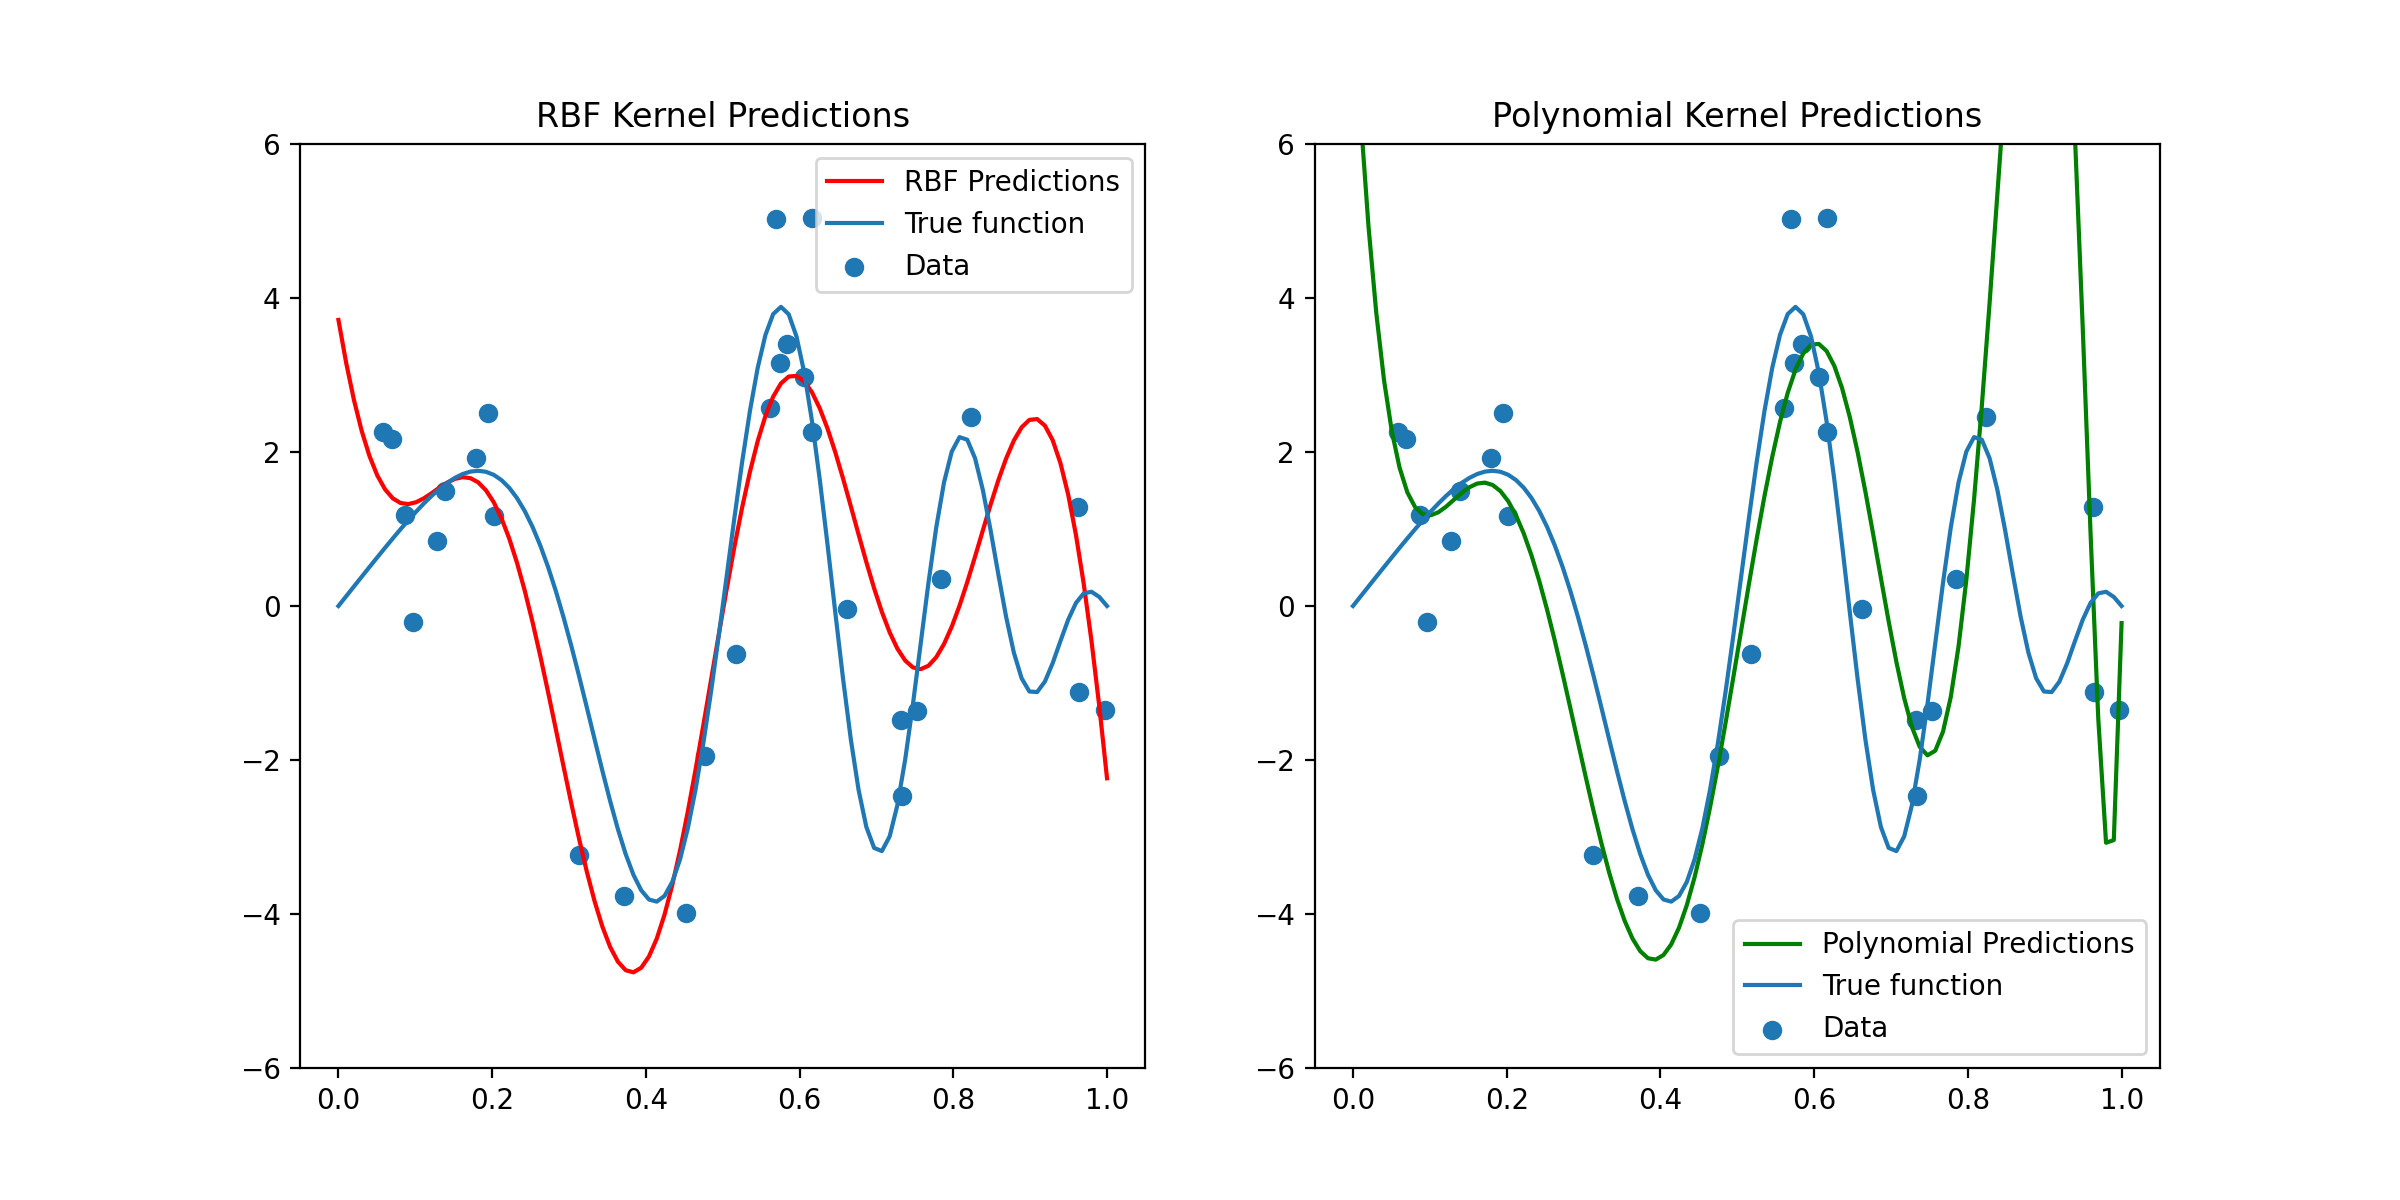
\includegraphics[width=.9\linewidth]{kernel.png}
            \caption{A3}
            \label{fig:kernel}
        \end{figure*}
    \end{itemize}
\end{aprob}


\section*{Perceptron}
% \begin{bprob}
%     One of the oldest algorithms used in machine learning (from the early 60's) is an online algorithm for learning a linear threshold function called the Perceptron Algorithm.
%     It works as follows:
%     \begin{enumerate}[label=\arabic*.]
%         \item Start with the all-zeroes weight vector $\mathbf{w}_1 = 0$, and initialize $t$ to $1$. Also let's automatically scale all examples $\mathbf{x}$ to have (Euclidean) norm $1$, since this doesn't affect which side of the plane they are on.
%         \item Given example $\mathbf{x}$, predict positive iff $\mathbf{w}_t \cdot \mathbf{x} > 0$.
%         \item On a mistake, update as follows:
%         \begin{itemize}
%             \item Mistake on positive: $\mathbf{w}_{t+1} \leftarrow \mathbf{w}_t + \mathbf{x}$. 
%             \item Mistake on negative: $\mathbf{w}_{t+1} \leftarrow \mathbf{w}_t - \mathbf{x}$.
%         \end{itemize}
%         \item $t \leftarrow t + 1$.
%     \end{enumerate}
%     If we make a mistake on a positive $\mathbf{x}$ we get $\mathbf{w}_{t + 1} \cdot \mathbf{x} = (\mathbf{w}_{t} + \mathbf{x}) \cdot \mathbf{x} = \mathbf{w}_{t} \cdot \mathbf{x} + 1$, and similarly if we make a mistake on a negative $\mathbf{x}$ we have $\mathbf{w}_{t + 1} \cdot \mathbf{x} = (\mathbf{w}_{t} - \mathbf{x}) \cdot \mathbf{x} = \mathbf{w}_{t} \cdot \mathbf{x} - 1$. So, in both cases we move closer (by 1) to the value we wanted. Here is a \href{https://en.wikipedia.org/wiki/Perceptron}{link} if you are interested in more details.\\
    
%     Now consider the linear decision boundary for classification (labels in $\{-1,1\}$) of the form
%     $\mathbf{w}\cdot \mathbf{x} = 0$ (i.e., no offset).
%     Now consider the following loss function evaluated at a data point $(\mathbf{x}, y)$ which is a variant on the hinge loss.
%     $$\ell((\mathbf{x},y), \mathbf{w})  = \max \{ 0, -y (\mathbf{w}\cdot \mathbf{x})\}.$$
%     \begin{enumerate}
%         \item \points{2} Given a dataset of $(\mathbf{x}_i,y_i)$ pairs, write down a single step of subgradient descent with a step size of $\eta$ if we are trying to minimize
%         $$\frac{1}{n}\sum_{i=1}^n \ell((\mathbf{x}_i,y_i), \mathbf{w})$$
%         for $\ell(\cdot)$ defined as above. That is, given a current iterate $\widetilde{\mathbf{w}}$ what is an expression for the next iterate?  
%         \item \points{2} Use what you derived to argue that the Perceptron can be viewed as implementing SGD applied to the loss function just described (for what value of $\eta$)?
%         \item \points{1} Suppose your data was drawn i.i.d. and that there exists a $\mathbf{w}^*$ that separates the two classes perfectly. Provide an explanation for why hinge loss is generally preferred over the loss given above. Murphy, Chapter 17.3 (Support vector machines) will be helpful here.
%     \end{enumerate}
    
%     \subsection*{What to Submit:}
%     \begin{itemize}
%         \item \textbf{Part a:} Expression for a single step of subgradient descent
%         \item \textbf{Part b:} A 1-2 sentence explanation.
%         \item \textbf{Part c:} A 1-2 sentence explanation.
%     \end{itemize}
% \end{bprob}

\section*{Introduction to PyTorch}
  \subsection*{Resources}
        For questions A.4 and A.5, you will use PyTorch.
        In Section materials (Week 6) there is a notebook that you might find useful.
        Additionally make use of \href{https://pytorch.org/docs/stable/index.html}{PyTorch Documentation}, when needed.
        
        % If you do not have access to GPU, you might find \href{https://colab.research.google.com/}{Google Colaboratory} useful.
        % It allows you to use a cloud GPU for free.
        % To enable it make sure: "Runtime" -> "Change runtime type" -> "Hardware accelerator" is set to "GPU". When submitting please download and submit a \texttt{.py} version of your notebook.

\begin{aprob}
    \label{code-pytorch}
    PyTorch is a great tool for developing, deploying and researching neural networks and other gradient-based algorithms.
    In this problem we will explore how this package is built, and re-implement some of its core components.
    Firstly start by reading \texttt{README.md} file provided in \texttt{intro\_pytorch} subfolder.
    A lot of problem statements will overlap between here, readme's and comments in functions.
    
    \begin{enumerate}
        \item \points{10} You will start by implementing components of our own PyTorch modules. You can find these in folders: \texttt{layers}, \texttt{losses} and \texttt{optimizers}. Almost each file there should contain at least one problem function, including exact directions for what to achieve in this problem. Lastly, you should implement functions in \texttt{train.py} file.
        \item \points{5} Next we will use the above module to perform hyperparameter search. Here we will also treat loss function as a hyper-parameter. However, because cross-entropy and MSE require different shapes we are going to use two different files: \texttt{crossentropy\_search.py} and \texttt{mean\_squared\_error\_search.py}.
        For each you will need to build and train (in provided order) 5 models:
        \begin{itemize}
            \item Linear neural network (Single layer, no activation function)
            \item NN with one hidden layer (2 units) and sigmoid activation function after the hidden layer
            \item NN with one hidden layer (2 units) and ReLU activation function after the hidden layer
            \item NN with two hidden layer (each with 2 units) and Sigmoid, ReLU activation functions after first and second hidden layers, respectively
            \item NN with two hidden layer (each with 2 units) and ReLU, Sigmoid activation functions after first and second hidden layers, respectively
        \end{itemize}
        For each loss function, submit a plot of losses from training and validation sets. All models should be on the same plot (10 lines per plot), with two plots total (1 for MSE, 1 for cross-entropy).
        \item \points{5} For each loss function, report the best performing architecture (best performing is defined here as achieving the lowest validation loss at any point during the training), and plot its guesses on test set. You should use function \texttt{plot\_model\_guesses} from \texttt{train.py} file. Lastly, report accuracy of that model on a test set.
    \end{enumerate}
    
    \subsubsection*{The Softmax function}
    One of the activation functions we ask you to implement is softmax. For a prediction $\hat{y} \in \mathbb{R}^k$ corresponding to single datapoint (in a problem with $k$ classes):
    \begin{align*}
        \text{softmax}(\hat{y}_i) = \frac{\exp(\hat{y}_i)}{\sum_j \exp(\hat{y}_j)}
    \end{align*}
    
    \subsubsection*{What to Submit:}
    \begin{itemize}
        \item \textbf{Part b:} 2 plots (one per loss function), with 10 lines each, showing both training and validation loss of each model. Make sure plots are titled, and have proper legends.
        \item \textbf{Part c:} Names of best performing models (i.e. descriptions of their architectures), and their accuracy on test set.
        \item \textbf{Part c:} 2 scatter plots (one per loss function), with predictions of best performing models on test set.
        \item \textbf{Code} on Gradescope through coding submission
    \end{itemize}
\end{aprob}

\section*{Neural Networks for MNIST}

\begin{aprob}
    \label{code-nn-mnist}
    In Homework 1, we used ridge regression to train a classifier for the MNIST dataset.
    In Homework 2, we used logistic regression to distinguish between the digits 2 and 7.
    Now, in this problem, we will use PyTorch to build a simple neural network classifier for MNIST to further improve our accuracy.\\\\
    We will implement two different architectures: a shallow but wide network, and a narrow but deeper network. For both architectures,
    we use $d$ to refer to the number of input features (in MNIST, $d=28^2 = 784$), $h_i$ to refer to the dimension of the $i$-th hidden layer and $k$ for the number of target classes (in MNIST, $k=10$). For the non-linear activation, use ReLU. Recall from lecture that
    \[ \text{ReLU}(x) = \begin{cases} 
          x, & x \geq 0 \\
          0, & x < 0 \ .
       \end{cases}
    \]
    \subsubsection*{Weight Initialization}
    Consider a weight matrix $W \in \mathbb{R}^{n \times m}$ and $b \in \mathbb{R}^n$. Note that here $m$ refers to the input dimension and
    $n$ to the output dimension of the transformation $x \mapsto Wx + b$. Define $\alpha = \frac{1}{\sqrt{m}}$.
    Initialize all your weight matrices and biases according to $\text{Unif}(-\alpha, \alpha)$.
    
    \subsubsection*{Training}
    For this assignment, use the Adam optimizer from \texttt{torch.optim}. Adam is a more advanced form of gradient descent that combines momentum and learning rate scaling. It often converges faster than regular gradient descent in practice. You can use either Gradient Descent or any form of Stochastic Gradient Descent. Note that you are still using Adam, but might pass either the full data, a single datapoint or a batch of data to it. Use cross entropy for the loss function and ReLU for the non-linearity.
    \subsubsection*{Implementing the Neural Networks}
    \begin{enumerate}
        \item \points{10}
        Let $W_0 \in \mathbb{R}^{h \times d}$, $b_0 \in \mathbb{R}^h$, $W_1 \in \mathbb{R}^{k \times h}$, $b_1 \in \mathbb{R}^k$ and $\sigma(z)\colon \mathbb{R} \to \mathbb{R}$
        some non-linear activation function applied element-wise. Given some $x \in \mathbb{R}^{d}$, the forward pass of the wide, shallow network can be formulated as:
        $$\mathcal{F}_1(x) \coloneqq W_1 \sigma(W_0 x + b_0) + b_1$$
        Use $h=64$ for the number of hidden units and choose an appropriate learning rate.
        Train the network until it reaches $99\%$ accuracy on the training data and provide a training plot (loss vs. epoch).
        Finally evaluate the model on the test data and report both the accuracy and the loss.
        \item \points{10}
        Let $W_0 \in \mathbb{R}^{h_0 \times d}$, $b_0 \in \mathbb{R}^{h_0}$, $W_1 \in \mathbb{R}^{h_1 \times h_0}$, $b_1 \in \mathbb{R}^{h_1}$,
        $W_2 \in \mathbb{R}^{k \times h_1}$, $b_2 \in \mathbb{R}^{k}$ and $\sigma(z) : \mathbb{R} \rightarrow \mathbb{R}$
        some non-linear activation function. Given some $x \in \mathbb{R}^{d}$, the forward pass of the network can be formulated as:
        $$\mathcal{F}_2(x) \coloneqq W_2 \sigma(W_1 \sigma(W_0 x + b_0) + b_1) + b_2$$
        Use $h_0 = h_1 = 32$ and perform the same steps as in part a.
        \item \points{5}
        Compute the total number of parameters of each network and report them.
        Then compare the number of parameters as well as the test accuracies the networks achieved. Is one of the approaches (wide, shallow vs. narrow, deeper) better than the other? Give
        an intuition for why or why not.
    \end{enumerate}
    
    \textcolor{red}{\textbf{Using PyTorch:}} For your solution, you may not use any functionality from the \texttt{torch.nn} module except for \texttt{torch.nn.functional.relu} and \texttt{torch.nn.functional.cross\_entropy}. You must implement the networks $\mathcal{F}_1$ and $\mathcal{F}_2$ from scratch. For starter code and a tutorial on PyTorch refer to the sections 6 and 7 material.
    \subsection*{What to Submit:}
    \begin{itemize}
        \item \textbf{Parts a-b:} Provide a plot of the training loss versus epoch. In addition, evaluate the model trained on the test data and report the accuracy and loss.
        \item \textbf{Part c:} Report the number of parameters for the network trained in part (a) and for the network trained in part (b).  Provide a comparison of the two networks as described in part (c) in 1-2 sentences.
        \item \textbf{Code} on Gradescope through coding submission.
    \end{itemize}
    \begin{itemize}
        \item F1 Test Accuracy: 0.975, F1 Test Loss: 0.0847005844116211
        \item F2 Test Accuracy: 0.9678, F2 Test Loss: 0.14048632979393005
        \item F1 Total Parameters: 50890, F2 Total Parameters: 26506
        \item Despite having nearly twice as many parameters, the F1 model performs better than the F2 model. This might indicate that for the MNIST dataset, having more parameters in a single hidden layer is more beneficial than distributing them across multiple layers.
    \end{itemize}
    \begin{figure}[!h]
        \begin{subfigure}{.45\textwidth}
            \centering
            \includegraphics[width=.9\linewidth]{f1.png}
            \caption{F1}
            \label{fig:f1}
        \end{subfigure}
        \begin{subfigure}{.45\textwidth}
            \centering
            \includegraphics[width=.9\linewidth]{f2.png}
            \caption{F2}
            \label{fig:f2}
        \end{subfigure}
        \caption{A5}
    \end{figure}
\end{aprob}

\section*{Administrative}
\begin{aprob}
\begin{enumerate}
    \item \points{2} About how many hours did you spend on this homework? There is no right or wrong answer :)
    \item ~ 50 hours.
\end{enumerate}
    
\end{aprob}

\end{document}